\documentclass{../notatki}

\title{Języki formalne}

\begin{document}

\tableofcontents

\section{Literatura}

\begin{itemize}
    \item \href{}{J.E. Hopencroft "Wprowadzenie do teorii automatów i obliczeń"}
    \item \href{}{M. Sipser "Wprowadzenie do teorii obliczeń"}
    \item \href{}{G.E. Revesz "Introduction to formal languages"}
    \item \href{}{H.R. Lewin, Papadimitriou "Elements of the Theory of Computation"}
\end{itemize}

\section{Język}

$$
\infty \text{ zdań} + n \text{ reguł} = \text{język}
$$

\subsection{Funkcje języka}

\begin{enumerate}
    \item Poznawcza
    \item Społeczna
    \item Ekspresywna
\end{enumerate}

\subsection{Nauka o języku}

\begin{enumerate}
    \item syntaktyka - budowa
    \item semantyka - co znaczy?
    \item pragmatyka - jak się używa?
\end{enumerate}
Przykład:$2 + 3 \cdot 4$: różna semantyka $\rightarrow$ wieloznaczność syntaktyczna

\subsection{Definicja}

Język składa się z gramatyk i automatów. Gramatyka generuje język, automat rozpoznaje język.

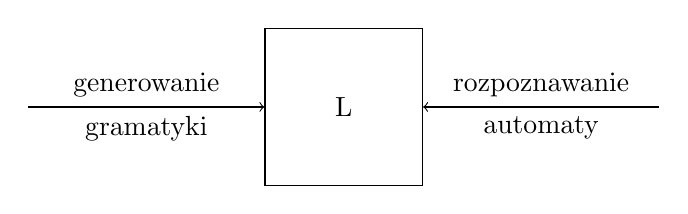
\begin{tikzpicture}[node distance=2cm]
    \node[draw, minimum size=2cm] (square) {L};
    \draw[<-] (square.west) -- node[anchor=south]{generowanie} node[anchor=north]{gramatyki} ++(-3,0);
    \draw[<-] (square.east) -- node[anchor=south]{rozpoznawanie} node[anchor=north]{automaty} ++(3,0);
\end{tikzpicture}

\section{Alfabet}

Alfabet to zbiór atomowych dozwolonych symboli

Przykład: $\{a, b, c, d\}$

\section{Słowo}

Słowo to skończony ciąg symboli nad alfabetem.

\begin{itemize}
    \item $\varepsilon$ - słowo puste
    \item $\{K, L, O, P, S\} \ne "KLOPS"$, ponieważ słowa mają dodane znaczenie, w postaci tego do którego języka należą.
\end{itemize}

\subsection{Konkatenacja}

\begin{itemize}
    \item $\text{Dla } P=a_1...a_n \text{ i } Q=b_1...b_n, \text{ to } PQ=a_1...a_nb_1...b_n$
    \item $P\epsilon = P$
    \item $\epsilon\epsilon = \epsilon$
\end{itemize}

\subsection{Podsłowo}

\begin{itemize}
    \item $P = Q_1 | Q | Q_2$
    \item $Q \subset P$
\end{itemize}

\subsection{Długość słowa}

\begin{itemize}
    \item $|\epsilon| = 0$
    \item $|Pa| = |P| + 1$
    \item $|PQ| = |P| + |Q|$
\end{itemize}

\subsection{Potęga słowa}

\begin{itemize}
    \item $P^0 = \epsilon$
    \item $P^{n + 1} = P^nP$
\end{itemize}

\subsection{Odbicie}

\begin{itemize}
    \item $\epsilon^-1 = \epsilon$
    \item $(Pa)^-1 = aP^-1$
\end{itemize}

\section{Język}

Zbiór dozwolonych słów nad alfabetem.

\begin{itemize}
    \item $V^*$ - zbiór wszystkich języków
    \item $V^+ = V^* \ {\epsilon}$
    \item $L \in V^*$
    \item $\{a, ab\} \ne {\epsilon, a, ab}$ ponieważ inaczej operacje na językach by nie działały
\end{itemize}

\subsection{Konkatenacja języków}

$$
L_1 = \{a, aa\}, L_2 = \{b, aba\}, L_1L_2 = \{ab, aaba, aab, aaaba\}
$$

\begin{table}[h!]
\centering
\begin{tabular}{c|c|c}
\backslashbox{$L_2$}{$L_1$} & a    & aa \\ \hline
b   & ab   & aab \\
aba & aaba & $aaaba$ \\
\end{tabular}
\caption{Tabela konkatenacji języków $L_1$ i $L_2$}
\end{table}

$|L_1L_2| \le |L_1| \cdot |L_2|$ bo eps wszystko psuje

$$
L_1 = \{a^n : n \ge 0\}, L_2 = \{b^n : n \ge 0\}, L_1L_2 = \{a^nb^m : n, m \ge 0\}
$$

\subsection{Potęga języka}

$$
L = \{a, ab\}, L^0 = \{\epsilon\}, L^1 = \{a, ab\}, L^2 = L \cdot L
$$

\textbf{Potęgowanie na językach jest dziwne}

$$
L = \{a^n : n \ge 0\}, L^2 = \{a^n a^m : a, m \ge 0\} = \{a^n : a \ge 0\} = L
$$

Potęgowanie języku \textbf{nie} zwiększyło mocy

$$
L = \{a^n : n > 0\}, L^2 = \{a^n a^m : a, m > 0\} = L \setminus \{a\} = \{a^n : n > 1\}
$$

Potęgowanie języku \textbf{zmniejszyło} moc

\subsection{Dzielenie słów}

$$
P \in L^n \rightarrow \text{ można podzielić } P \text{ na } n \text{ (niekoniecznie różnych) słów}
$$

$$
L = \{a, ab\}, "aababaabab" \in L^n, n=?
$$

Jest to problem wykładniczy, który wymaga stworzenia drzewa różnych możliwości.

\section{Domknięcie Kleenego}

$$
L^* = \bigcup_{n \ge 0}^{\infty}L^n
$$

$$
L^+ = \bigcup_{n \ge 1}^{\infty}L^n
$$

$$
L_1 = \{a\}, L_1^* = \{a^n : n \ge 0\}, L_1^+ = \{a^n : n > 0\}
$$

$$
L_2 = \{\epsilon, a\}, L_2^* = \{a^n : n \ge 0\} = L_2^+
$$

$$
L = \{aa, ab, ba, bb\}, L^* = \{P \in \{a, b\}^* : 2 | |P|\} = \text{wszystkie słowa nad alfabetem {a, b} o parzystej długości}
$$

\begin{itemize}
    \item $L^+ \subset L^*$
    \item $\epsilon \in L \rightarrow L^+ = L^*$
    \item $(L^*)^* = L^*$
    \item $L_1 \subset L_2 \rightarrow L_1^* \subset L_2^*$
\end{itemize}

$$
L = \{a^n : n > 1\}, L^1 \ne L^2, L^* = L
$$

\section{Automaty}

\begin{itemize}
    \item nieskończona taśma
    \item rejestry
    \item w każdym rejestrze symbol z alfabetu T
    \item głowica, która porusza się od lewej do prawej po rejestrach taśmy, aż do momentu, kiedy napotka pusty rejestr. Głowica zawsze jest w jednym ze stanów z zbioru stanów
\end{itemize}

\subsection{Deterministyczne automaty skończone}

Automat skończenie stanowy jest uporządkowaną piątką 
$$
\mathfrak{A} = \langle K,T,\delta,q_0,H \rangle 
$$

\begin{itemize}
    \item $K$   zbiór stanów
    \item $T$   alfabet - symbole z tego alfabetu znajdują się w rejestrach
    \item $\delta: K \times T \rightarrow K$  funkcja przejścia automatu
    \item $q_0$ stan początkowy automatu
    \item $H$ zbiór stanów akceptowalnych/końcowych
\end{itemize}

\subsubsection{Funkcja przejść}

Zbiory $K$ i $T$ są skończone, co oznacza, że funkcję $\delta$ można przedstawić w formie tabelki. Przykład:

$$
K = \{q_0, q_1, q_2\}, T = \{a,b\}, H = \{q_2\}
$$

$$
\delta: K \times T \rightarrow K
$$

\begin{figure}[h!]
    \centering
    \resizebox{0.5\textwidth}{!}{    
        \begin{minipage}{0.25\textwidth}
            \begin{tabular}{c|c|c}
                \backslashbox{$K$}{$T$} & a    & b \\ \hline
                $\rightarrow q_0$ & $q_2$ & $q_1$ \\
                $q_1$             & $q_0$ & $q_1$ \\
                $\underline{q_2}$ & $q_1$ & $q_2$ \\
            \end{tabular}
        \end{minipage}
        \begin{minipage}{0.25\textwidth}
            \begin{tikzpicture}[shorten >=1pt,node distance=2cm,on grid,auto]
                \node[state,initial] (q_0)   {$q_0$}; 
                \node[state] (q_1) [below right=of q_0] {$q_1$}; 
                \node[state,accepting] (q_2) [above right=of q_0] {$q_2$}; 
                \path[->] 
                (q_0) edge [bend left] node {a} (q_2)
                    edge [bend left] node {b} (q_1)
                (q_1) edge [loop right] node {b} ()
                    edge [bend left] node {a} (q_0)
                (q_2) edge [loop right] node {b} ()
                    edge [bend left] node {a} (q_1);
            \end{tikzpicture}
        \end{minipage}
    }
    \caption{Tabela konkatenacji języków $L_1$ i $L_2$ oraz graf przejść automatu}
    \label{fig:automat:example}
\end{figure}

\subsubsection{Rozszerzona funkcja przejść}

$$
\stackrel{\wedge}{\delta}: K \times T^* \rightarrow K
$$

\begin{itemize}
    \item $\stackrel{\wedge}{\delta}(q, \epsilon) = q$
    \item $\stackrel{\wedge}{\delta}(q, Pa) = \delta(\stackrel{\wedge}{\delta}(q, P), a)$
\end{itemize}

\subsubsection{Przykład}

Narysuj diagram przejścia deterministycznego automatu skończenie stanowego $\mathfrak{A}$ w którym $T=\{0, 1\}, P \in L(\mathfrak{A})$ wtedy i tylko wtedy gdy w $P$ występuje na pierwszym od końca miejscu.

\begin{figure}[h!]
    \centering
    \begin{tikzpicture}[shorten >=1pt,node distance=2cm,on grid,auto] 
        \node[state,initial] (q_0)   {$q_0$}; 
        \node[state,accepting](q_1) [right=of q_0] {$q_1$};
        \path[->] 
        (q_0) edge [bend left] node {1} (q_1)
            edge [loop above] node {0} ()
        (q_1) edge [bend left] node {0} (q_0) 
            edge [loop below] node {1} ();
    \end{tikzpicture}
    \caption{Diagram przejścia automatu do wykrywania 1 na pierwszym miejscu od końca}
    \label{fig:automat:1end}
\end{figure}

Narysuj diagram przejścia deterministycznego automatu skończenie stanowego $\mathfrak{A}$ w którym $T=\{0, 1\}, P \in L(\mathfrak{A})$ wtedy i tylko wtedy gdy w $P$ występuje na drugim od końca miejscu 1.

\begin{figure}[h!]
    \centering
    \begin{tikzpicture}[shorten >=1pt,node distance=2.0cm,on grid,auto]
        \node[state,initial] (q_0)   {$q_0$}; 
        \node[state](q_1) [right=of q_0] {$q_1$};
        \node[state,accepting](q_2) [above right=of q_1] {$q_2$};
        \node[state,accepting](q_3) [below right=of q_1] {$q_3$};
        \path[->] 
        (q_0) edge   node {1} (q_1)
            edge  [loop above] node {0} ()
        (q_1) edge  [bend left] node {0} (q_3)
            edge  [bend left] node {1} (q_2)
        (q_2) edge  [loop above] node {1} ()
            edge  [bend left] node {0} (q_3)
        (q_3) edge  [bend left] node {1} (q_1)
            edge  [bend left] node {0} (q_0);
    \end{tikzpicture}
    \caption{Diagram przejścia automatu do wykrywania 1 na drugim miejscu od końca}
    \label{fig:automat:2end}
\end{figure}

Widać na diagramie \ref{fig:automat:2end} wprost zależność że w zależności od miejsca od końca na którym ma być jeden rośnie ilość stanów.
Ilość stanów maszyny $|K|$ do wykrywania 1 na $n$-tym miejscu od końca można wyrazić w następujący sposób: $|K| = 2^n$ 

\subsection{Niedeterministyczne automaty skończone}

\begin{itemize}
    \item zamiast jednego stanu początkowego jest zbiór stanów początkowych
    \item niedeterministyczna funkcja przejścia, która zwraca zbiór wyjściowych stanów
\end{itemize}

$$
\mathfrak{A} = \langle K,T,\delta,Q_0,H \rangle 
$$

gdzie oznaczenia są identyczne jak dla deterministycznego automatu z dwoma różnicami:

\begin{itemize}
    \item $\delta: K \times T \rightarrow a \in K$  funkcja przejścia automatu
    \item $Q_0$ zbiór stanów początkowych automatu
\end{itemize}

\begin{figure}[h!]
    \centering
    \begin{tikzpicture}[shorten >=1pt,node distance=2cm,on grid,auto] 
        \node[state,initial] (q_0)   {$q_0$}; 
        \node[state](q_1) [right=of q_0] {$q_1$};
        \node[state,accepting](q_2) [right=of q_1] {$q_2$};
        \path[->] 
        (q_0) edge  node {1} (q_1)
            edge  [loop above] node {0,1} ()
        (q_1) edge  node {0,1} (q_2);
    \end{tikzpicture}
    \caption{Niedeterministyczna wersja automatu $\mathfrak{A}$ z rysunku \ref{fig:automat:2end}}
    \label{fig:automat:2end-ndet}
\end{figure}

Jak widać zamiast 4 stanów potrzeba tylko 3, to dlatego, że dla wersji niedeterministycznej $|K| = n + 1$

\subsubsection{Rozszerzona funkcja przejść}

$$
\stackrel{\wedge}{\delta}: P(K) \times T^* \rightarrow P(K)
$$

\begin{itemize}
    \item $\stackrel{\wedge}{\delta}(A, \epsilon) = A$
    \item $\stackrel{\wedge}{\delta}(A, Pa) = \bigcup_{q \in \stackrel{\wedge}{\delta}(A, P)}\delta(q, a)$
\end{itemize}

$$
\stackrel{\wedge}{\delta}(\{p\}, a) = \delta(p, a)
$$

\subsubsection{Twierdzenie Scotta}

\begin{itemize}
    \item każdy \textbf{nie}deterministyczny automat skończony można zastąpić równoważnym deterministycznym automatem skończonym
    $$\mathfrak{L}_{ndet} \subset \mathfrak{L}_{det}$$
    \item każdy deterministyczny automat skończony można zastąpić równoważnym \textbf{nie}deterministycznym automatem skończonym
    $$\mathfrak{L}_{det} \subset \mathfrak{L}_{ndet}$$
    \item liczba stanów automatu deterministycznego jest wykładnicza w stosunku do liczby stanów automatu niedeterministycznego
\end{itemize}

$$\mathfrak{L}_{det} = \mathfrak{L}_{ndet}$$

Zatem co nam daje niedeterministyczność? Przede wszystkim prostotę, ale kosztem wykładniczej złożoności.

Narysuj diagram przejścia deterministycznego automatu skończenie stanowego $\mathfrak{A}$ w którym $T=\{a\}, P \in L(\mathfrak{A})$ wtedy i tylko wtedy gdy $(2 | |P|) \vee (3 | |P|)$.

\begin{figure}
    \centering
    \begin{tikzpicture}[shorten >=1pt,node distance=2cm,on grid,auto] 
        \node[state,initial,accepting] (q_0)   {$q_0$}; 
        \node[state](q_1) [above right=of q_0] {$q_1$};
        \node[state, accepting](q_2) [right=of q_1] {$q_2$};
        \node[state, accepting](q_3) [below right=of q_2] {$q_3$};
        \node[state,accepting](q_4) [below left=of q_3] {$q_4$};
        \node[state](q_5) [left=of q_4] {$q_5$};
        \path[->] 
        (q_0) edge  node {a} (q_1)
        (q_1) edge  node {a} (q_2)
        (q_2) edge  node {a} (q_3)
        (q_3) edge  node {a} (q_4)
        (q_4) edge  node {a} (q_5)
        (q_5) edge  node {a} (q_0);
    \end{tikzpicture}
    \caption{Diagram przejścia automatu do wykrywania słów o długości podzielnej przez 2 lub 3}
    \label{fig:automat:2or3}
\end{figure}

Jak widzimy na diagramie \ref{fig:automat:2or3} przyjmuje postać cyklu o okresie 6, ponieważ $NWW(3,2)=6$.
Problem z diagramami deterministycznym się pojawia dla wyższych liczb, np.: $7$ i $5$, wtedy $NWW(7,5)=35$.
Zatem narysujmy diagram niedeterministyczny \ref{fig:automat:5or7}.

\begin{figure}
    \centering
    \begin{tikzpicture}[shorten >=1pt,node distance=2cm,on grid,auto]
        \node[] (initial) {start};
        \node[state, accepting] (q5_0) [left=of initial] {$q_0^5$};
        \node[state] (q5_1) [below left=of q5_0] {$q_1^5$};
        \node[state] (q5_2) [left=of q5_1] {$q_2^5$};
        \node[state] (q5_4) [above left=of q5_0] {$q_4^5$};
        \node[state] (q5_3) [left=of q5_4] {$q_3^5$};
        
        \node[state, accepting] (q7_0) [right=of initial] {$q_0^7$};
        \node[state] (q7_1) [above right=of q7_0] {$q_1^7$};
        \node[state] (q7_2) [right=of q7_1] {$q_2^7$};
        \node[state] (q7_3) [right=of q7_2] {$q_3^7$};
        \node[state] (q7_6) [below right=of q7_0] {$q_6^7$};
        \node[state] (q7_5) [right=of q7_6] {$q_5^7$};
        \node[state] (q7_4) [right=of q7_5] {$q_4^7$};

        \path[->]
        (q5_0) edge node {a} (q5_1)
        (q5_1) edge node {a} (q5_2)
        (q5_2) edge node {a} (q5_3)
        (q5_3) edge node {a} (q5_4)
        (q5_4) edge node {a} (q5_0);


        \path[->]
        (q7_0) edge node {a} (q7_1)
        (q7_1) edge node {a} (q7_2)
        (q7_2) edge node {a} (q7_3)
        (q7_3) edge node {a} (q7_4)
        (q7_4) edge node {a} (q7_5)
        (q7_5) edge node {a} (q7_6)
        (q7_6) edge node {a} (q7_0);

        \draw[->] (initial) -- (q5_0);
        \draw[->] (initial) -- (q7_0);
    \end{tikzpicture}
    \caption{Diagram przejścia automatu ndet do wykrywania słów o długości podzielnej przez 5 lub 7}
    \label{fig:automat:5or7}
\end{figure}

Jako, że automaty niedetermnistyczne pozwalają na kilka stanów początkowych, to tworzymy diagram niespójny, który w zależności od tego czy $|P|$ jest podzielne przez $5$ czy $7$ przechodzi do odpowiedniego pod-automatu.
Najłatwiej to można sobie wyobrazić jako dwa równoległe automaty z alternatywą na koniec.

\subsubsection{Przekształcenie niedet \texorpdfstring{$\rightarrow$}{->} det}

$$
\mathfrak{A} = \langle K,T,\delta,Q_0,H \rangle
$$

$$
\mathfrak{A}' = \langle K',T',\delta',q_0',H' \rangle 
$$

$$
L(\mathfrak{A}) = L(\mathfrak{A}')
$$

\begin{itemize}
    \item $T' = T$ bo nie ma sensu zmieniać taśmy
    \item $K' = P(K)$ \textbf{Wykładniczy wzrost liczby stanów}\\
    w przekształceniu będziemy używać systemu etykiet(konstrukcja potęgowa) aby zamieniać zbiory stanów na pojedyncze stany
    $$
    \{q_0,q_1\} = q^{01}
    $$
    $$
    P(K) = \{q^\emptyset, q^1, q^0, q^{10}, ...\}
    $$
    \item $q_0' = Q_0$ - stan odpowiadający zbiorowi stanów początkowych
    \item $H' = \{A \in K' : A \cap H \ne \emptyset\}$
    \item $\delta'(A, a) = \bigcup_{q \in A}\delta(q, a)$
\end{itemize}

Dla automatu \ref{fig:automat:2end-ndet} zbudujmy równoważny automat deterministyczny.
Korzystając z powyższych zasad otrzymujemy:

\begin{itemize}
    \item $K' = P(K) = \{\emptyset, \{q_0\}, ..., \{q_1, q_2\}, \{q_0, q_1, q_2\}\} = \{q^\emptyset, q^0, ..., q^{12}, q^{012}\}$
    \item $H' = \{q^2, q^{12}, q^{02}, q^{012}\}$
    \item $q_0' = \{q_0\} = q^0$
\end{itemize}

\begin{figure}[h!]
    \centering
    \resizebox{0.5\textwidth}{!}{    
        
        \begin{minipage}{0.25\textwidth}
            \begin{tabular}{c|c|c}
                \backslashbox{$K'$}{$T$} & 0             & 1 \\ \hline
                $q^\emptyset$            & $q^\emptyset$ & $q^\emptyset$ \\
                $\rightarrow q^0$        & $q^0$         & $q^{01}$ \\
                $q^1$                    & $q^2$         & $q^2$ \\
                $\underline{q^2}$        & $q^\emptyset$ & $q^\emptyset$ \\
                $q^{01}$                 & $q^{02}$      & $q^{012}$ \\
                $\underline{q^{12}}$     & $q^2$         & $q^2$ \\
                $\underline{q^{02}}$     & $q^0$         & $q^{01}$ \\
                $\underline{q^{012}}$    & $q^{02}$      & $q^{012}$ \\
            \end{tabular}
        \end{minipage}
        \begin{minipage}{0.45\textwidth}
            \begin{tikzpicture}[shorten >=1pt,node distance=2cm,on grid,auto]
                \node[state,initial] (q_0)   {$q^0$}; 
                \node[state](q_1) [right=of q_0] {$q^{01}$};
                \node[state,accepting](q_2) [above right=of q_1] {$q^{012}$};
                \node[state,accepting](q_3) [below right=of q_1] {$q^{02}$};
                \node[state,accepting](q_4) [above right=of q_3] {$q^2$};
                \node[state](q_6) [right=of q_4] {$q^\emptyset$};
                \node[state](q_5) [above=of q_4] {$q^1$};
                \node[state,accepting](q_7) [below=of q_4] {$q^{12}$};
                \path[->] 
                (q_0) edge   node {1} (q_1)
                    edge  [loop above] node {0} ()
                (q_1) edge  [bend left] node {0} (q_3)
                    edge  [bend left] node {1} (q_2)
                (q_2) edge  [loop above] node {1} ()
                    edge  [bend left] node {0} (q_3)
                (q_3) edge  [bend left] node {1} (q_1)
                    edge  [bend left] node {0} (q_0)
                (q_4) edge node {0, 1} (q_6)
                (q_5) edge node {0, 1} (q_4)
                (q_7) edge node {0, 1} (q_4)
                (q_6) edge [loop above] node {0, 1} (q_6);
            \end{tikzpicture}
        \end{minipage}
    }
    \caption{Zdeterminizowany automat z rysunku \ref{fig:automat:2end-ndet} i jego tabela przejść}
    \label{fig:automat:2end-det}
\end{figure}

Jak widać na diagramie \ref{fig:automat:2end-det} liczba stanów wzrosła z 3 do 8, co jest zgodne z przewidywaniami.
Jednocześnie widać, że diagram \ref{fig:automat:2end} zawiera się w diagramie \ref{fig:automat:2end-det}, co niekoniecznie oznacza, że są sobie równoważne, lecz jako, że stany dodatkowe są nieosiągalne to te dwa automaty są równoważne.
\textbf{Nie zawsze równoważność automatów będzie tak oczywista.}

\subsection{Automaty z przejściem}

Co jeśli moglibyśmy zmienić stan ale nie ruszyć głowicy? Wtedy mamy do czynienia z automatem z przejściem.

$$
\epsilon \in T, \epsilon = \text{nie ruszaj głowicy automatu}
$$

$$
\delta: K \times (T \cup \{\epsilon\}) \rightarrow P(K)
$$

\textbf{Każdy automat z przejściem jest niedeterministyczny}

\begin{figure}[h!]
    \centering
    \begin{tikzpicture}[shorten >=1pt,node distance=2cm,on grid,auto] 
        \node[state,initial] (q_0)   {$q_0$}; 
        \node[state](q_1) [right=of q_0] {$q_1$};
        \node[state,accepting](q_2) [right=of q_1] {$q_2$};
        \path[->] 
        (q_0) edge  node {$\epsilon$} (q_1)
            edge  [loop above] node {0} ()
        (q_1) edge  node {$\epsilon$} (q_2)
            edge  [loop above] node {1} ();
    \end{tikzpicture}
    \caption{Automat z przejściem}
    \label{fig:automat:epsilon}
\end{figure}
Automat przedstawiony na rysunku \ref{fig:automat:epsilon} akceptuje języki o następującej postaci $L(\mathfrak{A})=\{0^n1^m2^k: n,m,k \ge 0\}$.

\textbf{Nie istnieją różne epsilony:} $00\epsilon1\epsilon222 = 00122$

\subsubsection{Domknięcie stanu}

$$
E(q) = \text{zbiór stanów osiągalnych z } q \text{ przez dowolną liczbę epsilonów}
$$

\begin{enumerate}
    \item $q \in E(q)$
    \item $r \in E(q) \wedge p \in \delta(r, \epsilon) \rightarrow p \in E(q)$
\end{enumerate}

\subsubsection{Domknięcie zbioru stanów}

$$
E(A) = \bigcup_{q \in A}E(q)
$$

\subsubsection{Rozszerzona funkcja przejść}

$$
\stackrel{\wedge}{\delta}: P(K) \times T^* \rightarrow P(K)
$$

\begin{itemize}
    \item $\stackrel{\wedge}{\delta}(A, \epsilon) = E(A)$
    \item $\stackrel{\wedge}{\delta}(A, Pa) = \bigcup_{q \in \stackrel{\wedge}{\delta}(A, P)}E(\delta(q, a))$
\end{itemize}

\subsubsection{Przekształcenie \texorpdfstring{$\epsilon \rightarrow$}{->} ndet}

$$
\mathfrak{A}' = \langle K',T',\delta',Q_0',H' \rangle
$$

$$
T' = T, K' = K, H' = H, Q_0' = E(Q_0), \delta'(A, a) = E(\delta(q, a))
$$

$$
\mathfrak{L_{ndet} = \mathfrak{L_{\epsilon}}}
$$

\subsection{Def języków akceptowalnych przez automaty ndet oraz z przejściem}

$$
L(\mathfrak{A}) = \{P \in T^* : \stackrel{\wedge}{\delta}(Q_0, P) \cap H \ne \emptyset\}
$$

\section{Wyrażenia regularne}

$$
Reg(V) = \text{zbiór wyrażeń regularnych nad alfabetem } V
$$

\begin{itemize}
    \item $o \in Reg(V)$
    \item $e \in Reg(V)$
    \item $a \in V \rightarrow a \in Reg(V)$
    \item $u, v \in Reg(V) \rightarrow (u + v), (u \cdot v), (u^*) \in Reg(V)$
\end{itemize}

\subsection{Operacje}

\textbf{W kolejności od najwyższego priorytetu do najniższego}

\begin{enumerate}
    \item $L(u^*) = (L(u))^*$
    \item $L(uv) = L(u) \cdot L(v)$
    \item $L(u + v) = L(u) \cup L(v)$
    \item $L(u) = \{u\}$
\end{enumerate}

\subsection{Przykłady}

$$
L(ba^*) = \{ba^n : n \ge 0\}
$$

$$
L(ba^*) = L(b)L(a^*) = \{b\} \cdot (L(a))^* = \{b\} \cdot \{a\}^* = \{ba^n : n \ge 0\}
$$

$L((a + b)^*ab(a + b)^*)$ - wszystkie słowa nad alfabetem $\{a, b\}$ zaczynające się od a i kończące się b

\end{document}
